\documentclass[10pt]{amsart}
\usepackage{geometry}                % See geometry.pdf to learn the layout options. There are lots.
\geometry{letterpaper}                   % ... or a4paper or a5paper or ... 
%\geometry{landscape}                % Activate for for rotated page geometry
%\usepackage[parfill]{parskip}    % Activate to begin paragraphs with an empty line rather than an indent
\usepackage{graphicx}
\usepackage{amssymb}
\usepackage{epstopdf}
\DeclareGraphicsRule{.tif}{png}{.png}{`convert #1 `dirname #1`/`basename #1 .tif`.png}

\title{5-stage detector calibration for proton Computed Tomography (pCT)}
\author{Valentina Giacometi}
\author{Nicholas Vence}
\author{Vladimir Bashkirov}
%\date{}                                           % Activate to display a given date or no date

\begin{document}
\maketitle


pCT is important because ...

The Loma Linda University pCT detector [CITE] is composed of a Tracker and 5-stage energy detector which optimizes the benefits of a range finder and a single crystal detector.
A range detector is mechanically more complex involving an array of (N ~ 100) stages (each a few millimeters thick) and silicon photomultiplier tubes.
This simplifies range detection by having the furthest downstream signal marks the range of the proton.
By contrast, the accuracy of a single-crystal detector (N = 1) is defined by its energy resolution ~0.5\%; however, this will be insufficient of achieving the desired accuracy of the Water Equivalent Path Lengths (WEPL): 1\% of the proton range, which is $\sigma$ = 2.7 mm for 200 MeV protons.
Therefore, we divided our energy detector into 5 stages to spatially localize the Bragg peak energy burst.

All detectors require calibration matching the incoming energy \& detector response to the WEPL traversed by the proton. To expedite this procedure, we created a special step (calibration) phantom [see Fig 1(a) \& (b)].

\begin{figure}[htbp] %  figure placement: here, top, bottom, or page
   \centering
   \includegraphics[width=2.0in]{pCT2.pdf}
   \includegraphics[width=2.0in]{pCT2pic.pdf}
   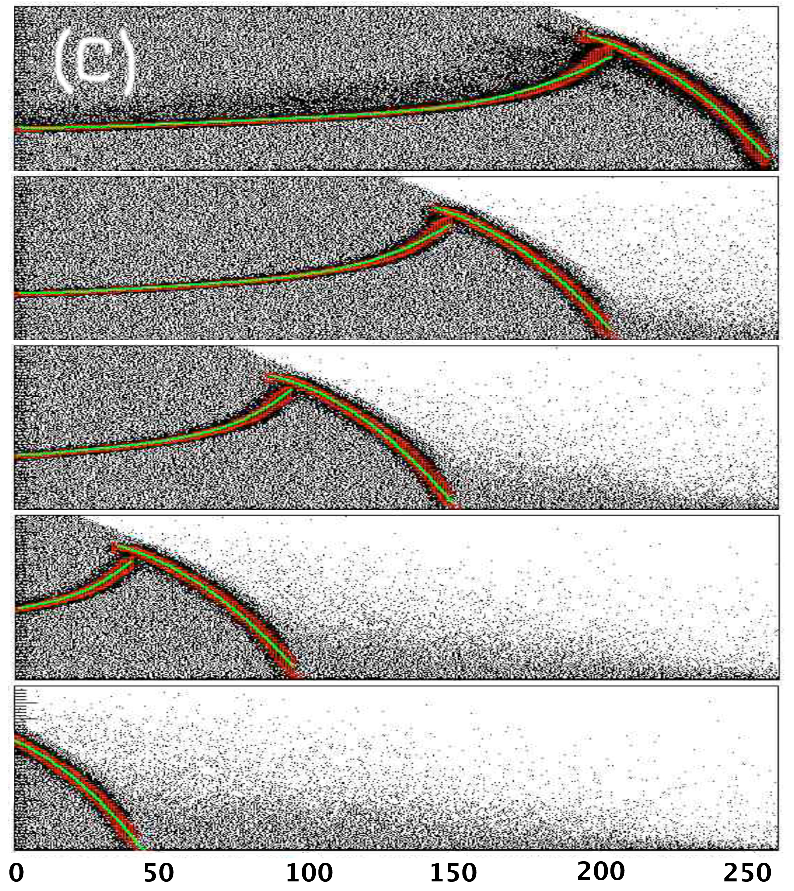
\includegraphics[width=1.5in]{Scatter.pdf} 
   \caption{(a) Geant4 representation of the 5-stage energy detector with calibration phantom between the front and rear tracker planes of pCT2. (b) response of individual stages as a function of the Water Equivalent Path Length.}
   \label{F:pic}
\end{figure}

Fig. 1(c) shows the response of the 5-stage detector as a function of WEPL in Monte Carlo simulation data.
The response of stopping-protons is seen by the curve to the right of the cusp, while the response of through-protons is shown by the curve to the left of the cusp.
While the stopping curve presents the most accurate results, the passing curve is useful for disambiguating protons stopping near the stage boundaries.
At periodic WEPL, we fit a Gaussian whose peak (green) and full-width half-maximum (red) mark the average values and their uncertainty.
A given detector response corresponds to one WEPL value (determined by the deepest stage) and an uncertainty in the range proportional to the slope (dWEPL/dResponse) of the response and dispersion of the data (thickness dWEPL of the red curve).
\begin{figure}[tbp] %  figure placement: here, top, bottom, or page
   \centering
   \includegraphics[width=5.5in]{WEPL_uncertainty.pdf} 
   \caption{Variation in range uncertainty vs WEPL for the experimental and Monte Carlo data.}
   \label{F:pic}
\end{figure}
Fig. 2 displays this uncertainty as a function of WEPL for the Monte Carlo \& experimental data.
As expected, the stopping curves have the lowest WEPL uncertainty (which was fit to a quartic polynomial), and upstream stages (with little variation in response) have the largest WEPL uncertainty.
The boundary cusp uncertainty (corresponding to the area between detectors) can be lowered by using a weighted average of detector measurements.
Interestingly, we obtain an optimum fit using information from two � not all of the fired stages.

\begin{figure}[htbp] %  figure placement: here, top, bottom, or page
   \centering
   \includegraphics[width=3.0in]{error.pdf}
   \includegraphics[width=2.0in]{WEPLresponse.pdf}
   \caption{WEPL uncertainty vs WEPL.}
   \label{F:pic}
\end{figure}
Fig. 3(a) combines the five fitting functions with the weighted mean response at the cusp to show the WEPL uncertainty vs WEPL.
This uncertainty is relatively constant with a periodic shift happening at ---.
Fig. 3(b) shows the final function used to reconstruct the WEPL from a given set of detector responses; this function provides a stable WEPL reconstruction whose accuracy is close to the straggling limits.

\end{document}  
